To understand if the solution works it will be subjected to a test with origin in the requirement specification \ref{sec:reqspec}. The requirements, which will be tested, are listed here:

\begin{enumerate}
\setlength{\itemsep}{0mm}
	\item Detect position of table.
	\item Detect position of balls.
	\item Identify balls with high accuracy.
	\item Identification and position of balls should be obtained within 1 second.
	\item Work with mixed light conditions and not only those stated in WPAB rules \ref{sec:rules}.
\end{enumerate}

The tests for the first four requirements will be done individually with the different locations and lighting as described in section \ref{sec:testsetup}. The fifth requirement will be tested within the other requirements by altering the light.

\subsection{Test setup}
\label{sec:testsetup}
The test are conducted in the multimedia lab located in room A6-314 on Niels Jernes Vej 12 in Aalborg where image and video material for the solution to this project were made. 

A second smaller test, to illustrate that the solution will work for different pool tables, is conducted in the DE-Klub which is a student bar located in A4-101 at Frederik Bajers Vej 7 in Aalborg. The pool tables can be seen in figure \ref{fig:diffpool}. The videos used for the test can be found on the CD-ROM enclosed with this report.
\fixme{CD-Rom}

\begin{figure}[H]
  \centering
  \subfloat[Pool table in multimedia lab.]{\label{fig:gull}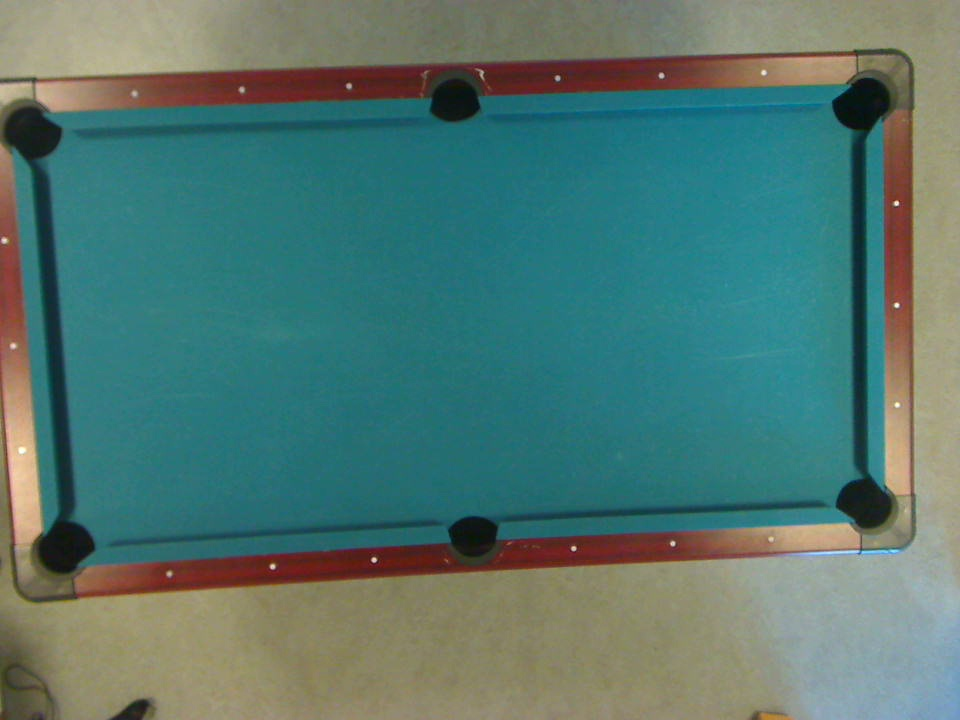
\includegraphics[width=0.48\textwidth]{images/test/light/input}}
  \quad           
%  \subfloat[Pool table in DE-Klub.]{\label{fig:tiger}\includegraphics[width=0.48\textwidth]{images/test/}}
   \caption{The two different pool tables used for testing.}
  \label{fig:diffpool}
\end{figure}

\fixme{Indsæt billeder}

The tests will be made in two light conditions: normal and mixed. These conditions can be seen in figure \ref{fig:difflightcon}. The reason for not doing it in dark conditions were because of the used webcams inability to regulate the exposure correctly.\\

\begin{figure}[H]
  \centering
  \subfloat[Normal illumination]{\label{fig:gull}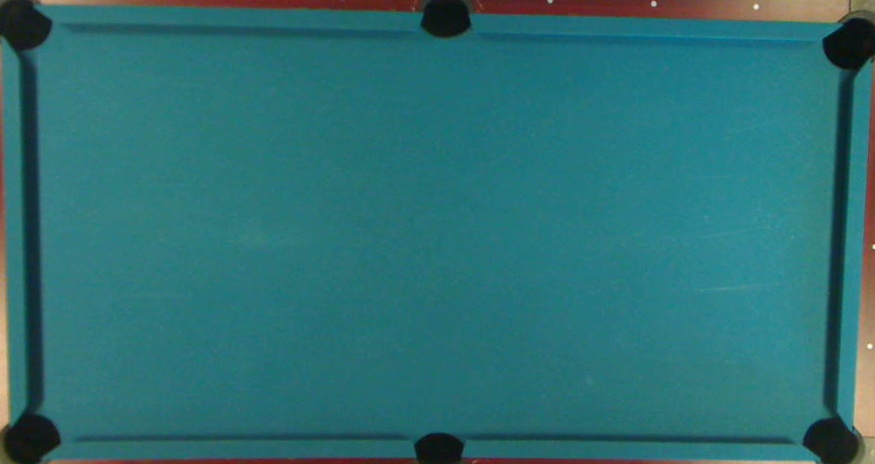
\includegraphics[width=0.48\textwidth]{images/test/light/detectedtable}}
  \quad           
%  \subfloat[Mixed illumination]{\label{fig:tiger}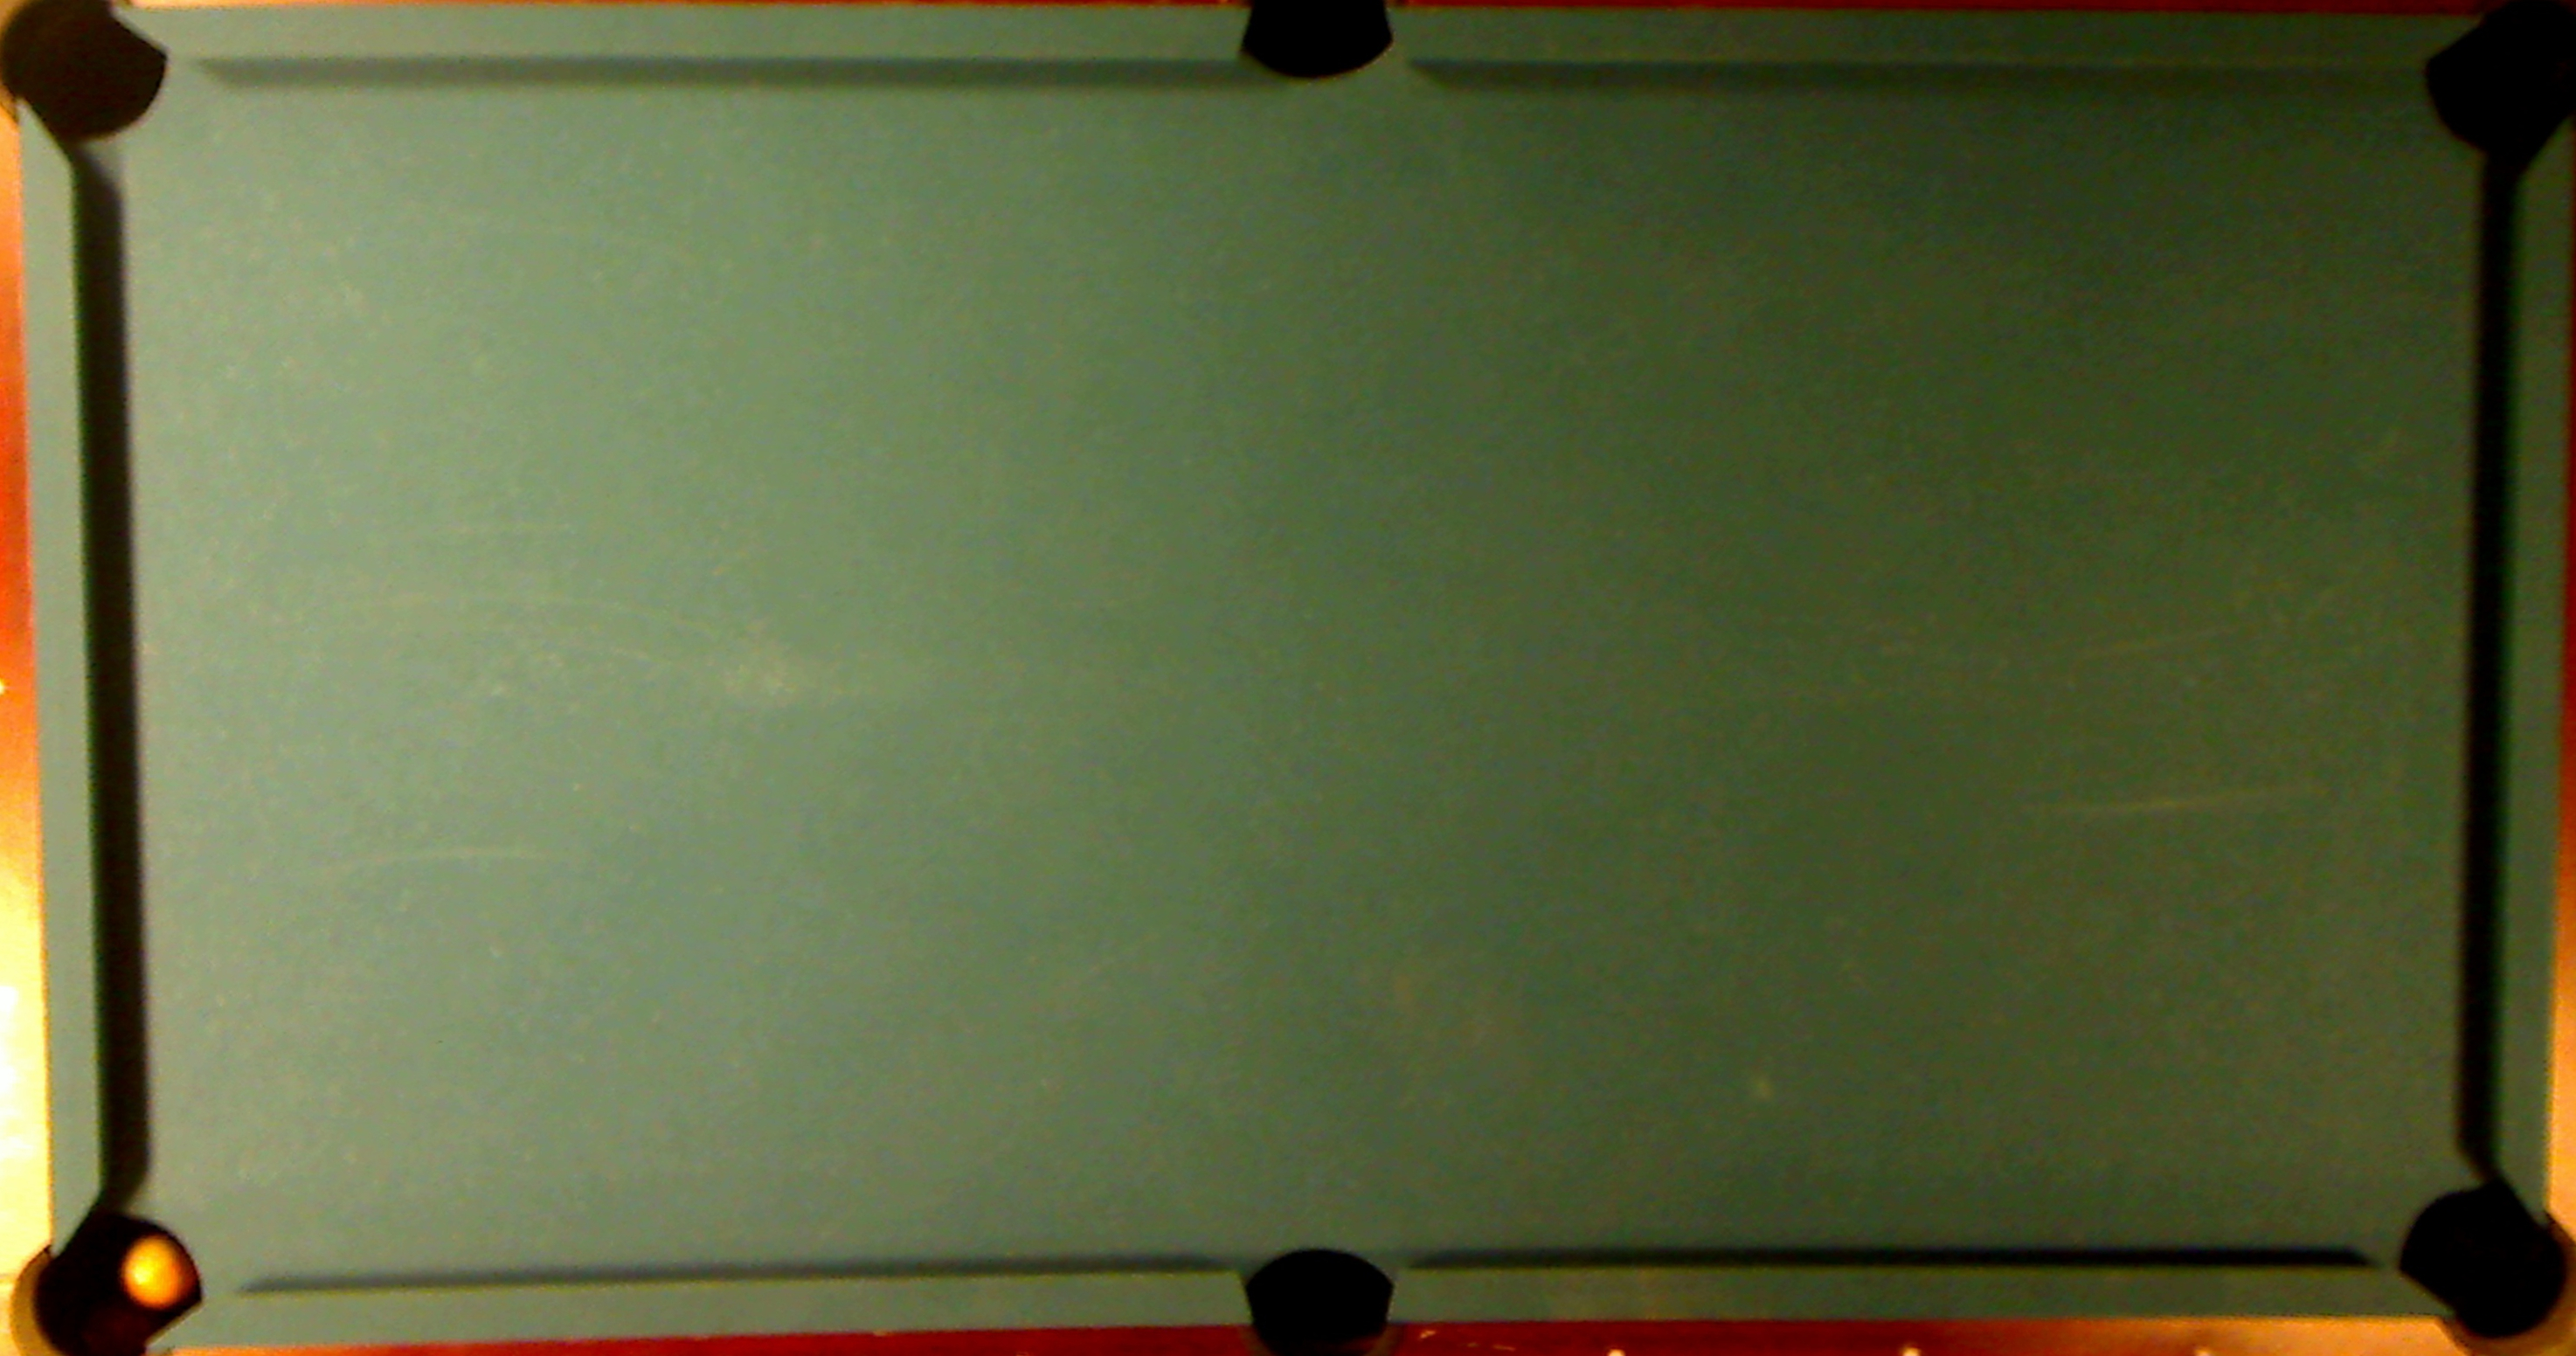
\includegraphics[width=0.48\textwidth]{images/test/mixed/detectedtable}}
   \caption{Table cloth in the two different light conditions.}
  \label{fig:difflightcon}
\end{figure}

\fixme{Indsæt billeder}

\subsection{1) Detect position of table}

This was tested numerous times and if the position of the table is within the view of the camera the table will be found in both light conditions.\\

\subsection{2) Detect position of balls}

The position of the balls is an important part of the project since the identification rests of being able to receive the correct information. Several different test have been concluded which is based on different positions and proximity of the balls.

\begin{enumerate}
\setlength{\itemsep}{0mm}
	\item Balls laying in start position as described in section \ref{sec:rules}.\\
	\item Balls laying apart.\\
	\item Balls laying in clusters where balls with similar colors are placed together.\\
\end{enumerate}

\subsubsection{ 1) Balls laying in start position}
The balls are placed in the start position with all balls except the cue ball clustered. This is the most difficult condition to test positions of the pool balls. The test was done while the balls were laying still and the result of the test with normal light can be seen in figure \ref{fig:poolposstart} and for the mixed light in figure \ref{fig:poolposstart2}.

\begin{figure}[H]
  \centering
   \subfloat[Correct detection]{\label{fig:tiger}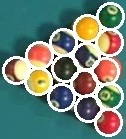
\includegraphics[width=0.4\textwidth]{images/test/light1/start-normal-1}}
\quad
   \subfloat[Incorrect detection]{\label{fig:tiger}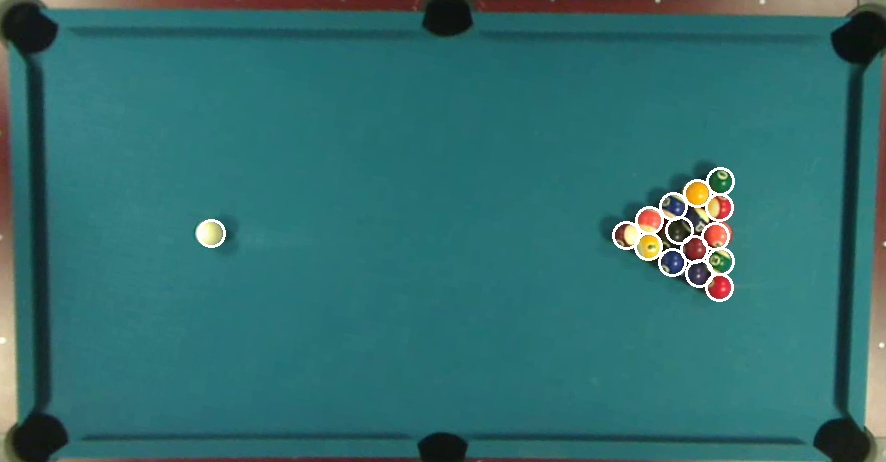
\includegraphics[width=0.4\textwidth]{images/test/light1/start-normal-2}}
   \caption{Pool balls in start position with normal light. The video used for testing is: start-normal.wmv}
  \label{fig:poolposstart}
\end{figure}

%Write conclusion

\begin{figure}[H]
  \centering
  \subfloat[Detection with incorrect position]{\label{fig:gull}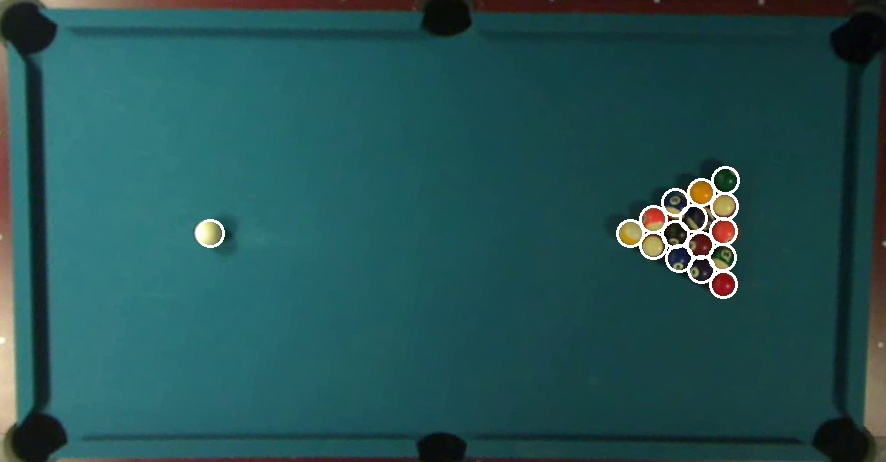
\includegraphics[width=0.4\textwidth]{images/test/mixed1/start-mixed-1}}
\quad
   \subfloat[One ball not detected]{\label{fig:tiger}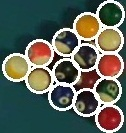
\includegraphics[width=0.4\textwidth]{images/test/mixed1/start-mixed-2}}
\quad
   \caption{Pool balls in start position with mixed light. The video used for testing is: start-mixed.wmv}
  \label{fig:poolposstart2}
\end{figure}

%Write conclusion

\subsubsection{ 2) Balls laying apart}
The least difficult test for the position of the balls is where the balls are laying apart. The result of the test with normal light can be seen in figure \ref{fig:apartnormal} and for the mixed light in figure \ref{fig:apartmixed}.

\begin{figure}[H]
  \centering
  \subfloat[Correct detection]{\label{fig:gull}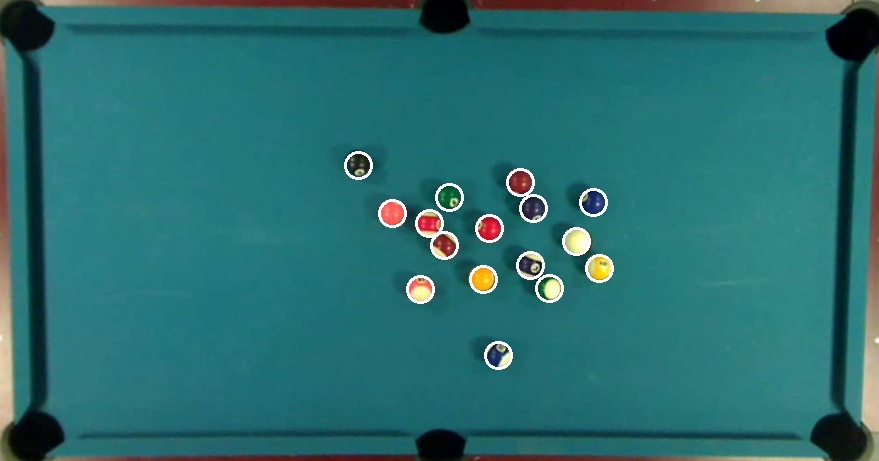
\includegraphics[width=0.5\textwidth]{images/test/light1/laying-apart}}
   \caption{Pool balls laying apart with normal light. The video used for testing is: balls-apart-normal.wmv}
  \label{fig:apartnormal}
\end{figure}

%Write conclusion

\begin{figure}[H]
  \centering
  \subfloat[Correct detection]{\label{fig:gull}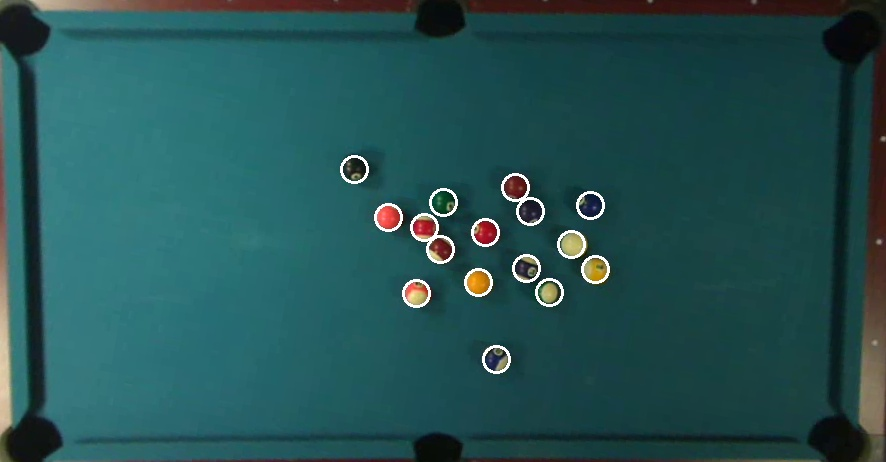
\includegraphics[width=0.5\textwidth]{images/test/mixed1/laying-apart}}
   \caption{Pool balls laying apart with mixed light.  The video used for testing is: balls-apart-mixed.wmv}
  \label{fig:apartmixed}
\end{figure}

%Write conclusion

\subsubsection{ 3) Balls laying in clusters where balls with similar colors are placed together}
Since the position method relies on bla bla  \fixme{noget om position og lidt varians}. The result of the test with normal light can be seen in figure \ref{fig:clustersnormal} and for the mixed light in figure \ref{fig:clustersmixed}.

\begin{figure}[H]
  \centering
  \subfloat[Mask for 8-ball laying placed wrong]{\label{fig:gull}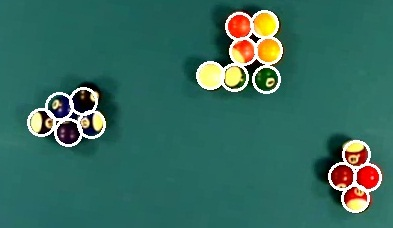
\includegraphics[width=0.5\textwidth]{images/test/light1/clusters-1}}
  \quad
   \subfloat[Two masks placed wrong]{\label{fig:tiger}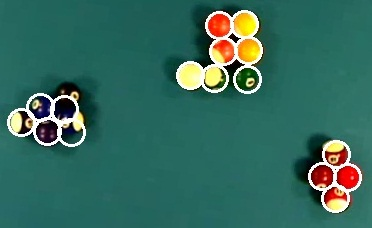
\includegraphics[width=0.5\textwidth]{images/test/light1/clusters-2}}
	\quad
   \caption{Pool balls laying in clusters with normal light. The video used for testing is: clusters-normal.wmv}
  \label{fig:clustersnormal}
\end{figure}

%Write conclusion

\begin{figure}[H]
  \centering
  \subfloat[Wrong detection]{\label{fig:gull}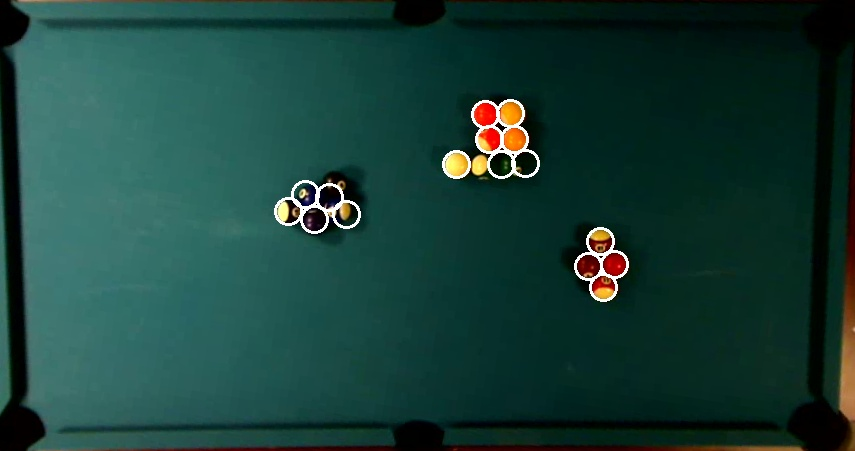
\includegraphics[width=0.5\textwidth]{images/test/mixed1/clusters-2}}
   \caption{Pool balls laying in clusters with mixed light.  The video used for testing is: clusters-mixed.wmv}
  \label{fig:clustersmixed}
\end{figure}

%Write conclusion

\subsection{3) Identify balls with high accuracy}

The identification of the balls is done by first calibrating the system and then running the different test scenarios which are as listed here:

\begin{enumerate}
\setlength{\itemsep}{0mm}
	\item Pool balls laying with maximum white facing up\\
	\item Pool balls laying with minimum white facing up\\
\end{enumerate}

\subsubsection{1) Pool balls laying with maximum white facing up}
This test will illustrate if the ratio of white pixels is defined well enough to identify if the ball is solid or striped. Also the detection of correct colors will be tested. The result of the test with normal light can be seen in figure \ref{fig:maxnormal} and for the mixed light in figure \ref{fig:maxmixed}.

\begin{figure}[H]
  \centering
  \subfloat[Input image]{\label{fig:gull}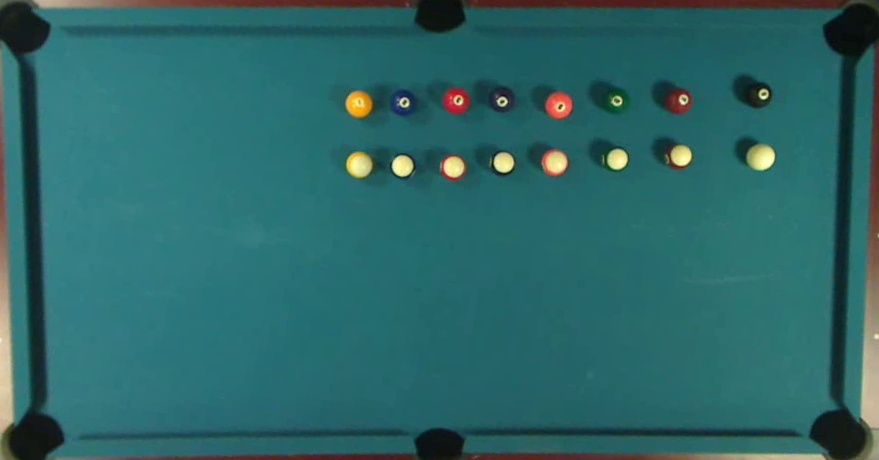
\includegraphics[width=0.5\textwidth]{images/test/light1/max-white-input}}
  \quad
   \subfloat[Found balls]{\label{fig:tiger}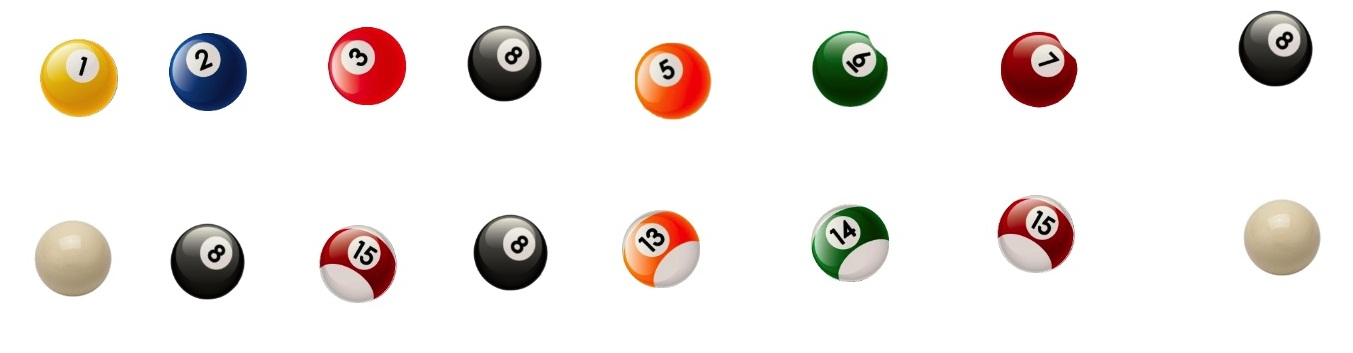
\includegraphics[width=0.5\textwidth]{images/test/light1/max-white-output}}
	\quad
   \caption{Pool balls laying with maximum white facing up and normal light. The video used for testing is: max-white-normal.wmv}
  \label{fig:maxnormal}
\end{figure}

%Write conclusion

\begin{figure}[H]
  \centering
  \subfloat[Input image]{\label{fig:gull}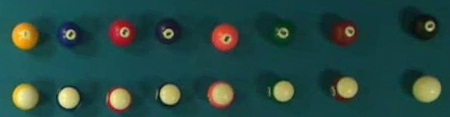
\includegraphics[width=0.5\textwidth]{images/test/mixed1/max-white-input}}
  \quad
  \subfloat[Found balls]{\label{fig:tiger}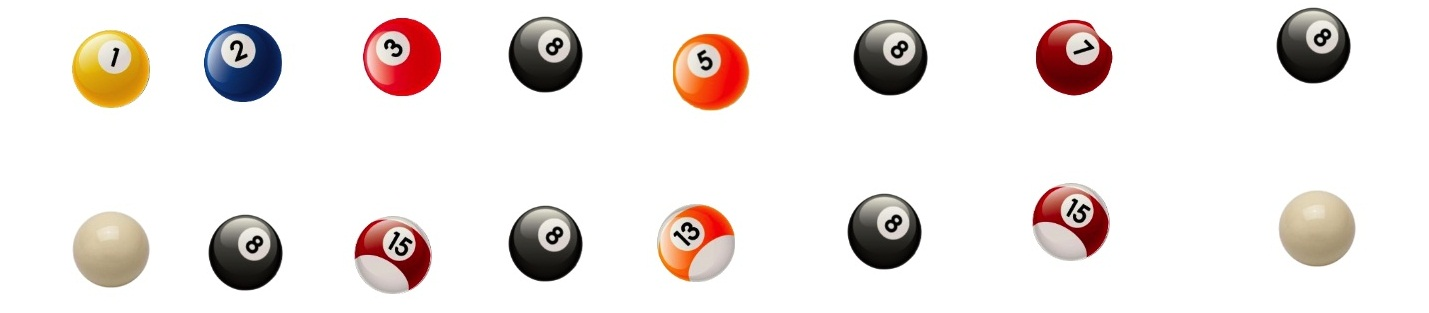
\includegraphics[width=0.5\textwidth]{images/test/mixed1/max-white-output}}
  \quad
   \caption{Pool balls laying with maximum white facing up and mixed light. The video used for testing is: max-white-mixed.wmv}
  \label{fig:maxmixed}
\end{figure}

%Write conclusion

\subsubsection{2) Pool balls laying with minimum white facing up}
%Write intro??
The result of the test with normal light can be seen in figure \ref{fig:minnormal} and for the mixed light in figure \ref{fig:minmixed}.

\begin{figure}[H]
  \centering
  \subfloat[Input image]{\label{fig:gull}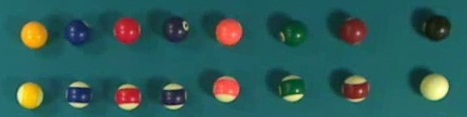
\includegraphics[width=0.5\textwidth]{images/test/light1/min-white-input}}
  \quad
   \subfloat[Found balls]{\label{fig:tiger}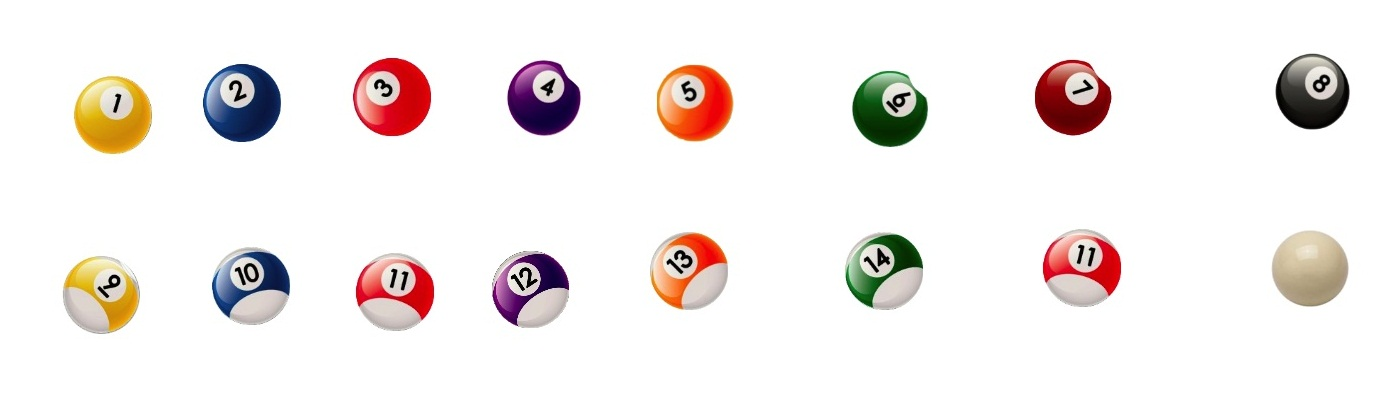
\includegraphics[width=0.5\textwidth]{images/test/light1/min-white-output}}
	\quad
   \caption{Pool balls laying with minimum white facing up and normal light. The video used for testing is: min-white-normal.wmv}
  \label{fig:minnormal}
\end{figure}

%Write conclusion

\begin{figure}[H]
  \centering
  \subfloat[Input image]{\label{fig:gull}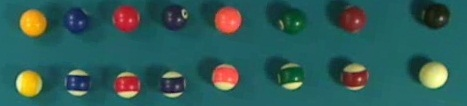
\includegraphics[width=0.5\textwidth]{images/test/mixed1/min-white-input}}
  \quad
  \subfloat[Found balls]{\label{fig:tiger}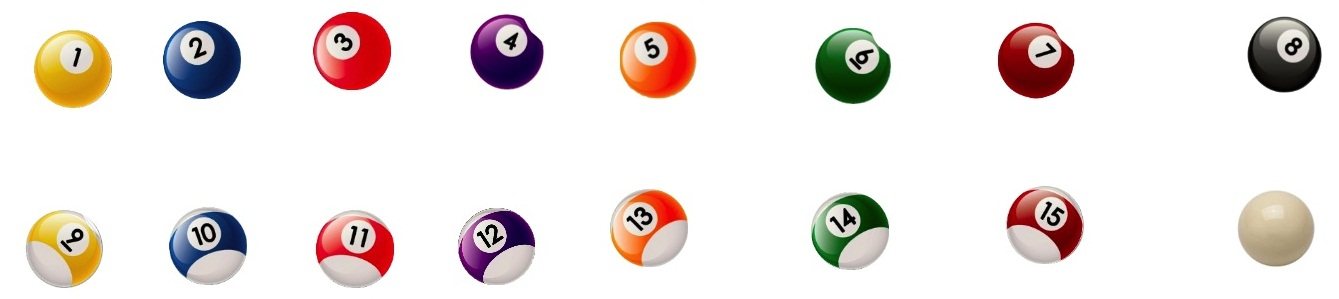
\includegraphics[width=0.5\textwidth]{images/test/mixed1/min-white-output}}
  \quad
   \caption{Pool balls laying with minimum white facing up and mixed light. The video used for testing is: min-white-mixed.wmv}
  \label{fig:minmixed}
\end{figure}


\subsection{4) Identification and position of balls should be obtained within 1 second}

Profile daz shit!
